Machine learning corresponds to the study and construction of systems that can learn from data. These systems can be useful when typical rule based programs that follow explicit instructions don't give good performance. Their ability to learn makes them popular in the field of artificial intelligence and patter recognition. Machine learning can take several forms. In this paper, we look specifically at classifiers within the field of supervised learning. In supervised learning the system is trained or "taught" using input data that is known to belong to a certain class of output. A typical methodology of training a classifier is displayed in figure \ref{fig:SL}. A mapping between the inputs and outputs is inferred from the training data which can be used to classify unseen data. \cite{cord2008machine}

In unsupervised learning, no associated label, which is the desired output for a set of inputs, is given to the learning algorithm. The class belonging to each instance in the dataset is unknown and there is no reward when the classifier picks the right class. This technique is therefore more often used when trying to discover hidden classes in new datasets \cite{maglogiannis2007emerging}.


\begin{figure}[H]
\centering
    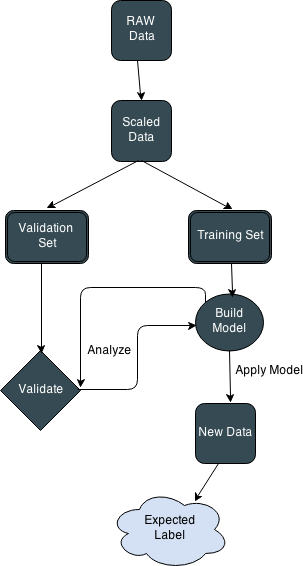
\includegraphics[width=38mm,scale=0.3]{./img/SL.png}
    \caption{\footnotesize{Supervised learning model}}
    \label{fig:SL}
\end{figure}



